\documentclass[border=8pt]{standalone}
\usepackage[T1]{fontenc}\usepackage[utf8]{inputenc}\usepackage{lmodern}
\usepackage{tikz}\usetikzlibrary{arrows.meta,positioning}
\begin{document}
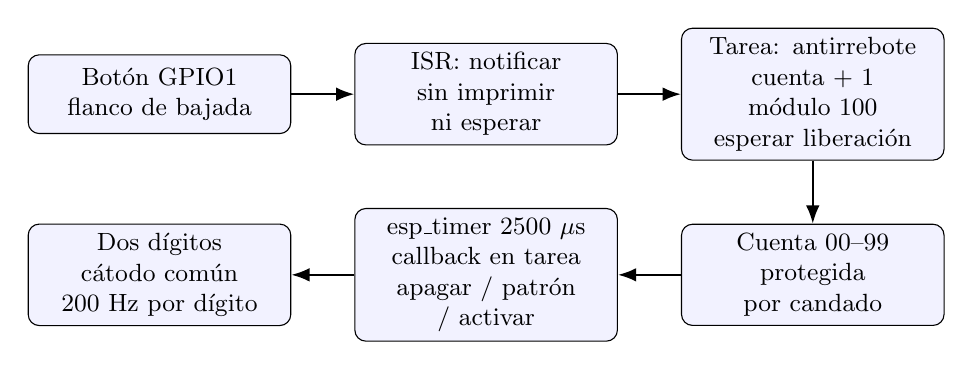
\begin{tikzpicture}[>=Latex,font=\small,node distance=0.8cm,
 b/.style={draw,rounded corners,fill=blue!5,text width=3.1cm,align=center,minimum height=1cm}]
\node[b] (btn) {Botón GPIO1\\flanco de bajada};
\node[b,right=of btn] (isr) {ISR: notificar\\sin imprimir ni esperar};
\node[b,right=of isr] (task) {Tarea: antirrebote\\cuenta + 1 módulo 100\\esperar liberación};
\node[b,below=of task] (data) {Cuenta 00--99\\protegida por candado};
\node[b,left=of data] (timer) {esp\_timer 2500 $\mu$s\\callback en tarea\\apagar / patrón / activar};
\node[b,left=of timer] (out) {Dos dígitos\\cátodo común\\200 Hz por dígito};
\draw[->,thick] (btn)--(isr);\draw[->,thick] (isr)--(task);\draw[->,thick] (task)--(data);
\draw[->,thick] (data)--(timer);\draw[->,thick] (timer)--(out);
\end{tikzpicture}
\end{document}
